
Basierend auf den Anforderungen (\autoref{sec:anforderungen}) an den zu entwickelnden Prototypen, wird im folgenden Abschnitt der zugrundeliegende Architektur-Entwurf ausgeführt. Die Ar\-chi\-tek\-tur-\-Ent\-schei\-dung\-en bilden die Grundlage für die Designentscheidungen des Soft\-wa\-re-\-Ent\-wurfs. Ausschlaggebend dafür ist das aus \cite{kruchten1995architectural} stammende \textit{4+1 Schichtenmodell}.


%\url{https://www4.in.tum.de/misc/perlen/perlen-folien/PDW_Architektur_IK_Druckversion.pdf}\\
%\url{http://www.edv-buchversand.de/chapter.php?cnt=getchapter&id=ha-41215_2.pdf}\\


\subsection{Kontextsicht}
    \begin{figure}[ht]
    \centering
    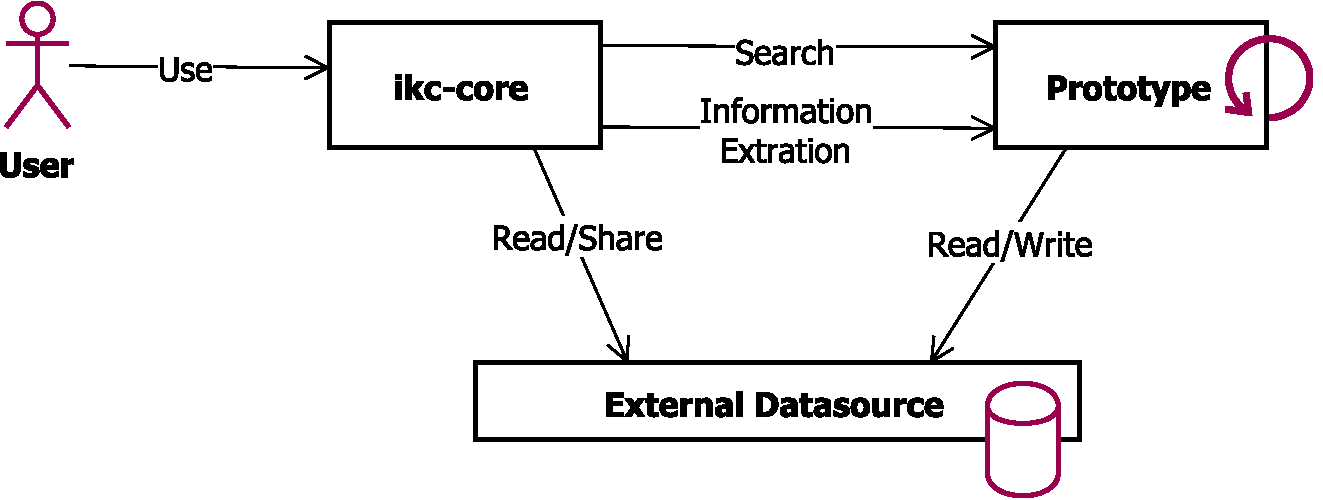
\includegraphics[width=1\textwidth]{BDA_Context}
    \caption{Kontextsicht}
    \label{fig:kontextsicht}
    \end{figure}
 
 Die \autoref{fig:kontextsicht} gibt einen Überblick über den Kontext des zu entwickelnden Prototypen:
 Der \texttt{ikc-core} nutzt den Prototypen zur Erweiterung seiner Funktionalität. Damit können die Hauptanforderungen, wie die Volltextsuche und die Extraktion von Schlüsselwörter, abgedeckt werden. Diese beiden Funktionen sind für den Benutzer über das \texttt{UserInterface} innerhalb des \gls{ikc-core} verfügbar. Sowohl der \gls{ikc-core} als auch der Prototyp haben Zugriff auf die externen Datenquellen. Der Prototyp hat dort die Quellen für die Dateiinhalte und hält dort auch Indizes für die Volltextsuche und die Schlü\-ssel\-wort-Ex\-trak\-tion.
 


%---------------------------------------------------------------------

\subsection{Einflussfaktoren}\label{einflussfaktoren}

%---------------------------------------------------------------------

Basierend auf dem Kontext des \gls{ikc-core}, dem Scope und den funktionalen und nichtfunktionalen Anforderungen beeinflussen verschiedenen Faktoren den Architektur-Entwurf.

\begin{longtable}{|p{4.2cm}|p{8.5cm}|}

  \hline
    Faktor &  Beschreibung \\\hline
    Browseranwendung & Der \gls{ikc-core} ist als clientseitige Browseranwendung aufgebaut und kann bis anhin grundsätzlich ohne serverseitige Logik genutzt werden. %Funktionale Erweiterungen mit Hilfe von zusätzlicher zentralen Services sind in Entwicklung. Diese betreffen jedoch keine grundlegenden Funktionen der Applikation.
    \\\hline
    Mehrplatz-Nutzung & Soll der \gls{ikc-core} in einer Mehrplatz-Umgebung genutzt werden, ist eine Synchronisation mit \gls{Dropbox} notwendig. Diese muss vom Benutzer explizit angegeben und autorisiert werden.\\\hline
    Hardware Infrastruktur & Die Server-Infrastruktur des Departements Informatik (\textit{enterpriselab}) bietet die Ressourcen, auf welchen die Webanwendung ausgeführt wird. Dazu werden zwei virtuelle \gls{Ubuntu}-Server verwendet. Die Entwicklung und die Produktion sind somit komplett voneinander getrennt.\\\hline
    
    Software Infrastruktur & Als Basis für Applikationsverteilung auf das Entwicklungs- und Produktions-System wird \gls{Dokku} in Kombination mit \gls{Gitlab CI} verwendet. Das Versionskontrollsystem verteilt Änderungen so direkt an die vorgesehende Infrastruktur. Die Software wird als \gls{Docker}-Container ausgeliefert und anschliessend als dedizierte Applikation innerhalb des \gls{Dokku}-Frameworks gestartet.\\\hline
    
    Programmiersprachen & Als Programmiersprache wird \gls{Typescript} verwendet. Anders als andere Webprogrammiersprachen wie \gls{Javascript} ermöglicht sie die Verwendung von Sprachkonstrukten der Typisierung, wie zum Beispiel Klassen oder Vererbung. Durch den Typescript-Kompiler wird der Code für die Ausführung in reinen \gls{Javascript} Code übersetzt. Mit der Verwendung der \gls{Node}-Plattform kann \gls{Typescript} auch für eine Server-Anwendung verwendet werden. Dadurch steigt sowohl die Wiederverwendbarkeit als auch Skalierbarkeit.\\\hline
    
    Kommunikation & Die allfällige Kommunikation zwischen dem \gls{ikc-core} und einer serverseitigen Erweiterung wird über einen Websocket abgehandelt. Dies ermöglicht beidseitige Kommunikation. \\\hline
    
    UI-Framework & Die Verwendung des \gls{React}-Frameworks ermöglicht den modularen Aufbau des \texttt{ikc-core}. Die gesamte Oberfläche ist in verschiedene Elemente aufgeteilt, welche über den Applikationzustand gesteuert werden. Eingaben des Benutzers werden durch die verschiedenen \texttt{UI Services} abgearbeitet und resultieren in einem aktualisierten Applikationszustand. Der unidirektionale Datenfluss sorgt für die klare Trennung der Verantwortlichkeiten innerhalb der \texttt{UI Services}. \\\hline
    
    Datenhaltung & Der \gls{ikc-core} nutzt keine zusätzlichen zentralen Services für die Persistenz von Benutzerdaten oder deren Applikations-Konfiguration. Es werden die lokalen Ressourcen oder externe Datenquellen wie \gls{Dropbox} verwendet. \\\hline
    \caption{Einflussfaktoren}
  \label{tab:einflussfaktoren}
\end{longtable}


%Der \gls{ikc-core} ist primär eine Browserapplikation, der Grossteil der verwendeten Komponenten läuft ebenfalls clientseitig. Die Kommunikation mit serverseitigen Services funktioniert über REST-Schnittstellen oder WebSockets. Darunter gehört beispielsweise eine Schnittstelle mit \gls{Evernote}. Dies hat insbesondere den Grund, dass durch die Nutzung des \gls{ikc-core} keine zusätzliche Persistenz eingeführt wird. Darum sind keine zentralen Applikations- und Datenserver notwendig.

%Dies schränkt die Architektur insoweit ein, dass Komponenten mit kritischer Funktionalität oder Leistung möglichst gekapselt und entkoppelt sind. Nur in diesem Fall ist gewährleistet, dass eine entsprechende Komponente, falls notwendig, auch auf einer Server-\-Um\-geb\-ung laufen kann.

%---------------------------------------------------------------------

\subsection{Architekturtreiber}

%---------------------------------------------------------------------

Drei elementare Architekturtreiber beeinflussen die Konzeption des Prototyps. Diese wurden teilweise bereits weiter oben als Einflussfaktor (\autoref{einflussfaktoren}) erwähnt, haben jedoch auch für den Prototyp eine zentrale Bedeutung.

\begin{itemize}
    \item \textbf{Entkopplung und Wiederverwendbarkeit}:
    Module und Komponenten sind entkoppelt voneinander. Dadurch können diese innerhalb der Applikation, oder auch für zukünftige Projekte, leicht wiederverwendet werden. Bei Performance-Engpässen ist es weiter möglich, bestimmte Module auszulagern, dies sowohl lokal innerhalb der Client-Applikation, als auch extern auf eine Server-Umgebung.
    \item \textbf{Verhinderung von zusätzlicher Persistenz}:
    Applikationsdaten und Konfiguration sind stets lediglich von den bestehenden Datenquellen zu beziehen. Hierbei handelt es sich entweder um den lokalen Cache des Benutzers oder die entsprechende externe Datenquelle. Durch diesen Umstand kann viel Zeit für die Entwicklung und die Absicherung einer Per\-si\-stenz-In\-fra\-struk\-tur gespart werden. Der Benutzer hat so zusätzlich immer eine transparente Kontrolle über den Speicherort und auch den Inhalt der eigenen Daten.
    \item \textbf{Inspiration durch React und Flux}: Wie in \autoref{react} bereits erwähnt, arbeitet React im Hintergrund mit einer eigenen Implementation von Flux. Dieser orientiert sich stark am funktionalen Programmier-Paradigma: Innere Zustände, also Variabeln, sind wann immer möglich zu verhindern. Dies wirkt allfälligen Seiteneffekten entgegen, macht den Code so nachvollziehbarer. Auch der unidirektionale Datenfluss strebt ähn\-liche Ziele an. Diese Überlegungen begleiteten die Entwicklung ständig. So sind an vielen Orten Programmierkonstrukte zu finden, welche prinzipiell verwandte Ansätze verfolgen.
\end{itemize}


%---------------------------------------------------------------------

\subsection{Architekturziele}

%---------------------------------------------------------------------

Der zu entwickelnde Prototyp baut auf dem bestehenden \gls{ikc-core} auf. Dabei soll das Augenmerk weiterhin auf den bereits bestehenden Eigenschaften der Architektur, insbesondere der Modularität und der Erweiterbarkeit, gehalten werden. Dies ist im Kontext des zugrundeliegenden Forschungsprojekts von hoher Wichtigkeit. Die Vergangenheit hat gezeigt, dass eine solide aber gleichzeitig auch anpassungsfähige Basis ein kritischer Faktor für die agile Weiterentwicklung ist. Einzig unter diesen Voraussetzungen ist es möglich, auf die stetig ändernden Anforderungen entsprechend zu reagieren.

Die wichtigsten Ziele der Architektur sind in folgender Tabelle (\autoref{tab:architekturziele}) kurz erläutert:

\begin{longtable}{|p{4.5cm}|p{8.5cm}|}

  \hline
    Ziel &  Beschreibung \\\hline
    Modularität & Die verschiedenen Komponenten sind auswechselbar und an anderen Orten wiederverwendbar. Eine lose Kopplung und eine hohe Kohäsion innerhalb der Komponenten und deren Klassen ist dafür vorausgesetzt.\\\hline
    Erweiterbarkeit & Die Komponenten sind offen für Erweiterungen. Ein Ausbau der Funktionalität ist stets möglich.\\\hline
    Skalierbarkeit & Durch Bildung von Schichten ist es möglich, einzelne Komponenten horizontal zu skalieren. Das bedeutet, dass mehrere gleiche Services sich beispielsweise einzelne Aufgaben teilen können. Dafür sind diverse Szenarien denkbar. Die Performance kann so gezielt an bestimmten Stellen optimiert werden.\\\hline
%    Vorbereitung Multiuser-Betrieb & \\\hline
    Benutzerfreundlichkeit & Bezüglich der Benutzeroberfläche ist es wichtig, dass der Benutzer immer über die Abläufe im Hintergrund informiert ist. Insbesondere bei der aufwändigen Verarbeitung von grossen Datenmengen ist der Benutzer nie gehindert oder gar blockiert, seine Arbeit mit dem Prototypen fortzusetzen. Sind die Resultate verfügbar, wird er benachrichtigt und kann auf deren Basis weiterarbeiten.\\\hline
    %Performance & \\\hline
    \caption{Ziele der Architektur}
  \label{tab:architekturziele}
\end{longtable}

% Performance, Stresstest, Flexibilität, Erweiterbarkeit, Benutzerfreundlichkeit
% anderer Kontext, ...
%Entkoppelt, einfach erweiterbar, modularisiert, microservices, skalierbar

%---------------------------------------------------------------------

\subsection{Bausteinsicht}

%---------------------------------------------------------------------

Die \autoref{fig:bausteinsicht} zeigt die Bausteinsicht der Architektur des Prototypen. Darin werden die verschiedenen Komponenten und Module und deren Beziehungen untereinander aufgezeigt. Hierbei werden drei verschiedene Abstraktionslevel unterschieden. 

\begin{figure}[H]
\centering
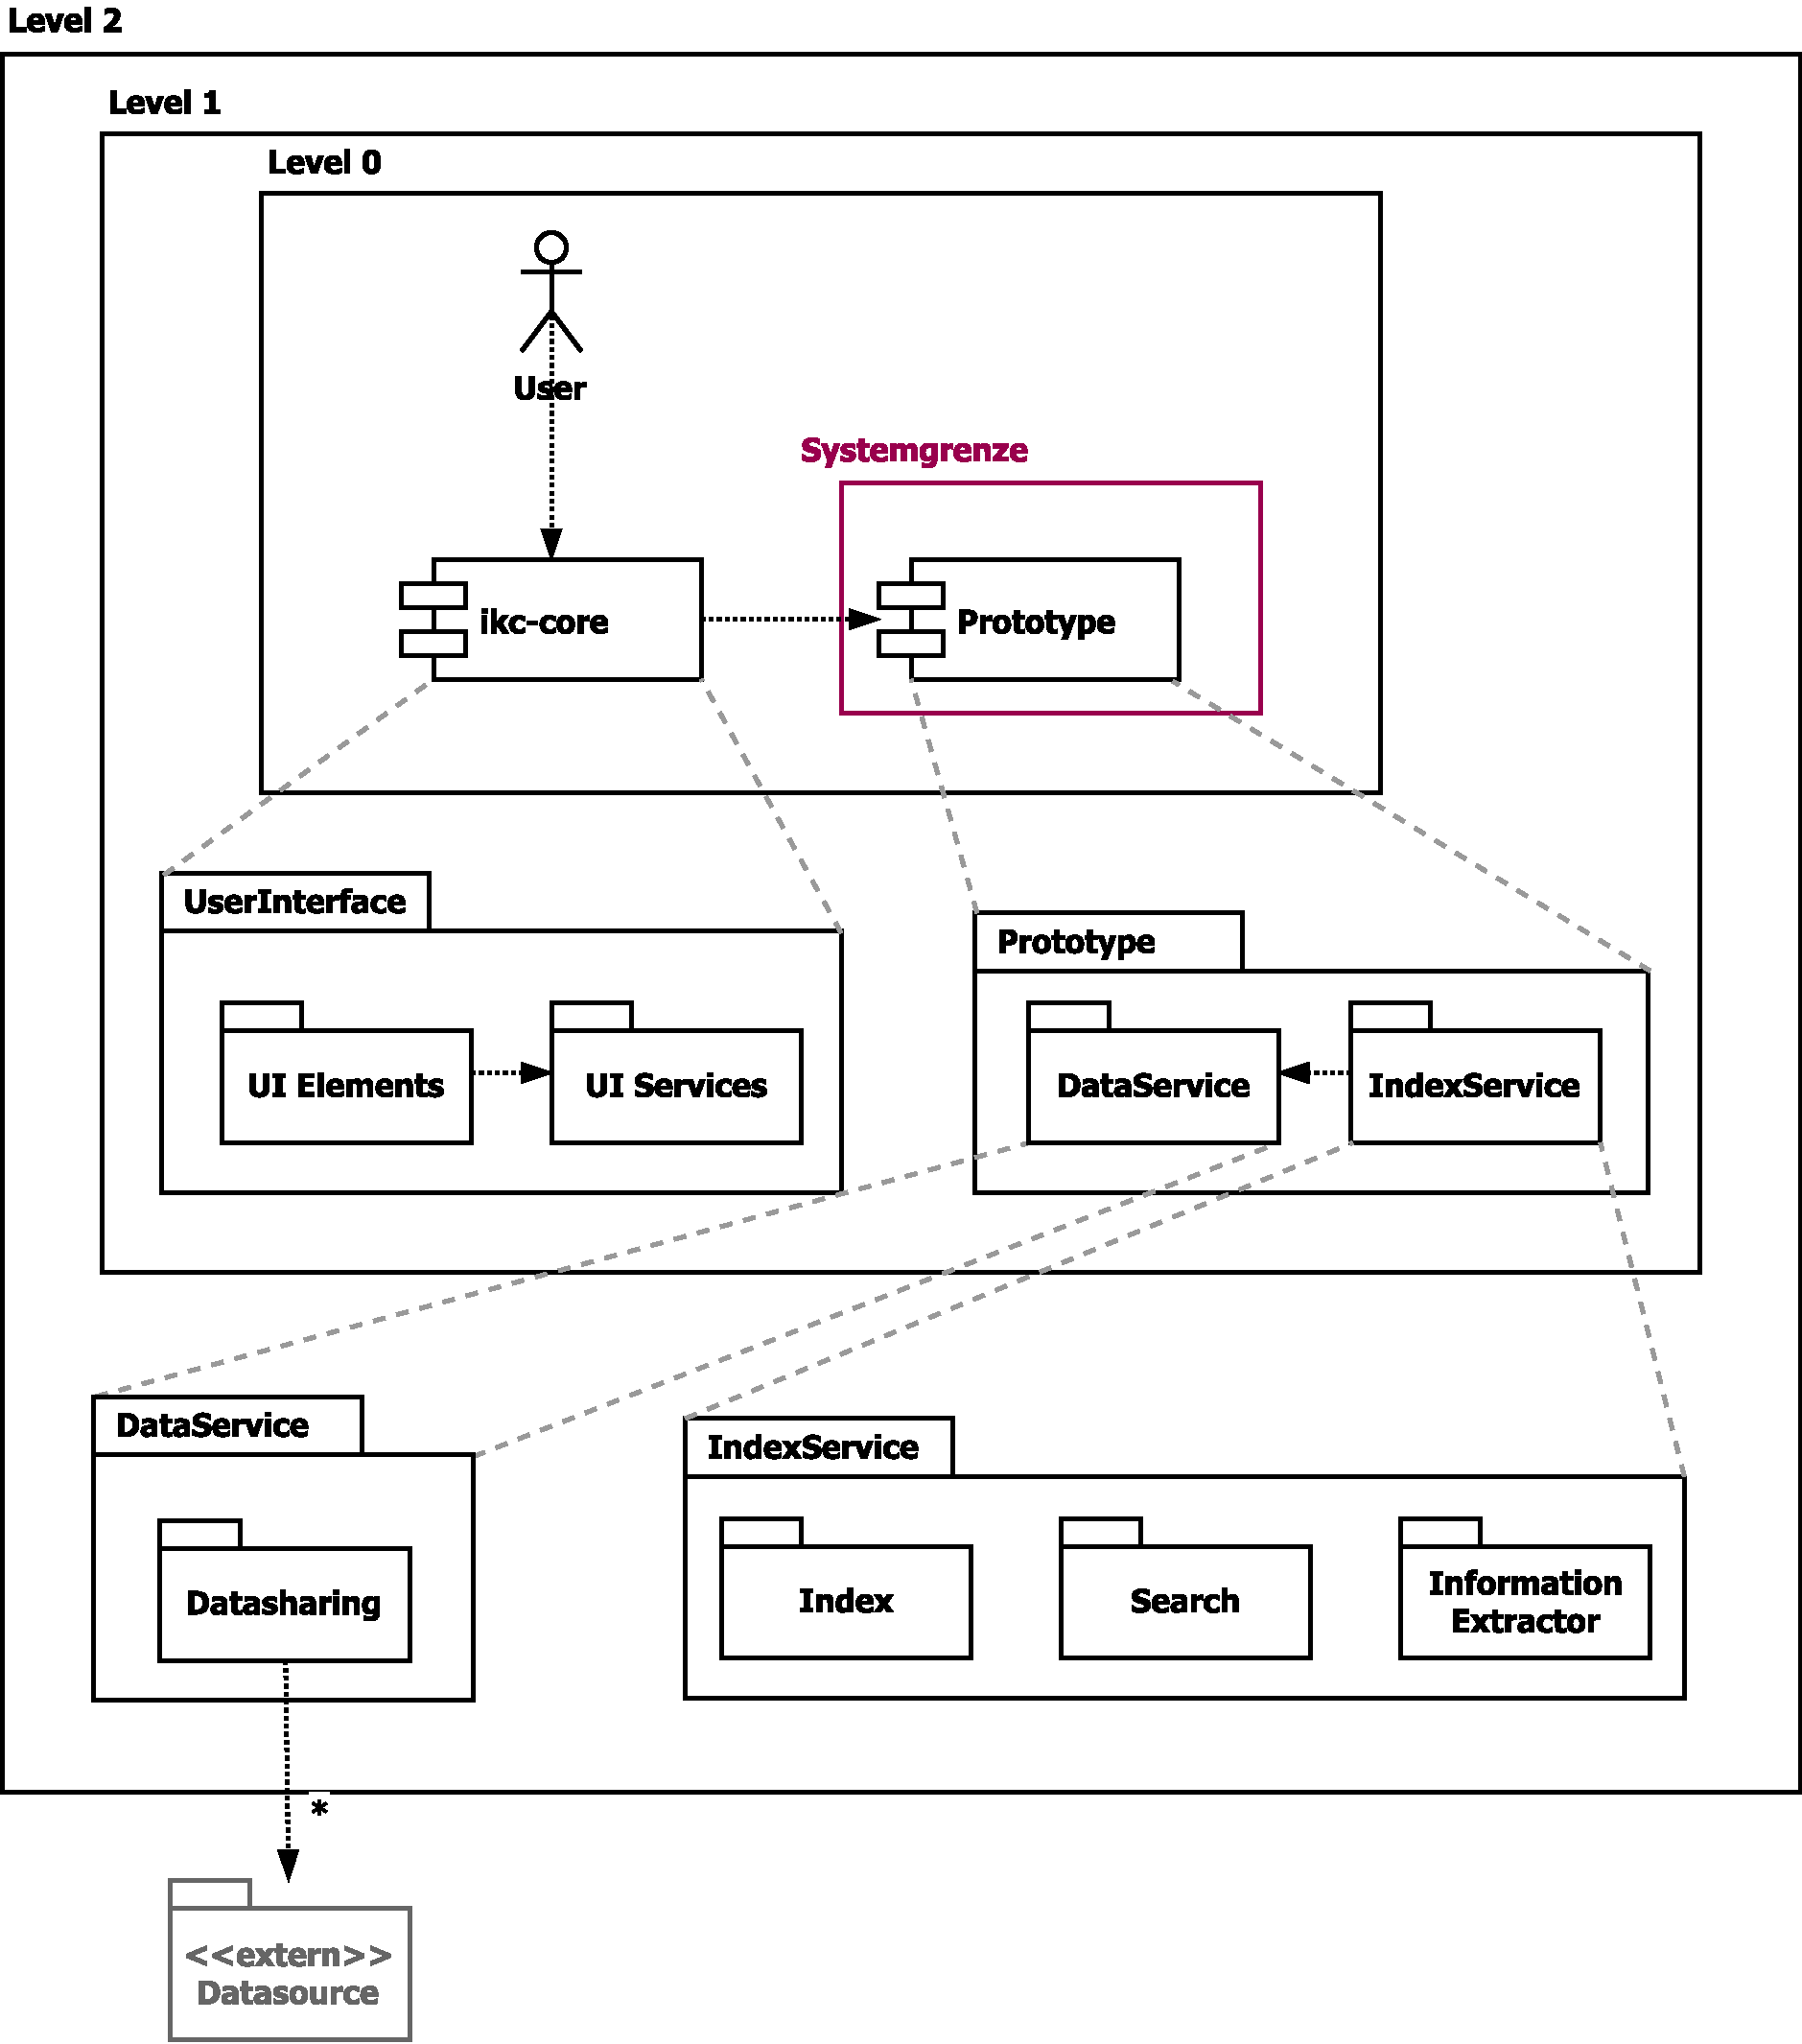
\includegraphics[width=1\textwidth]{BDA_Whitebox}
\caption{Bausteinsicht}
\label{fig:bausteinsicht}
\end{figure}

Nachfolgend werden diese näher erläutert.


%---------------------------------------------------------------------

\subsubsection{Bausteinsicht Level 0}

%---------------------------------------------------------------------

Innerhalb des \texttt{Level 0} werden die Zusammenhänge zwischen dem \texttt{User}, dem \texttt{ikc-core} und dem \texttt{Prototypen} aufgezeigt. Ebenfalls ist die Systemgrenze zwischen der bestehenden und der zu erstellenden Komponente ersichtlich. Die Systemgrenze grenzt den Kern des Prototyps ein.

%---------------------------------------------------------------------

\sssubsection{User}

%---------------------------------------------------------------------

Wie bisher hat der Benutzer über die Benutzeroberfläche des \gls{ikc-core} Zugriff auf die gesamte Funktionalität. Die Zusatzfunktionen, welche neu durch den Prototyp zur Verfügung gestellt werden, sind für den Benutzer in der Suchfunktion und den extrahierten Schlüsselwörtern ersichtlich.


%---------------------------------------------------------------------

\sssubsection{ikc-core}

%---------------------------------------------------------------------

Neben der bisherigen Funktionalität nutzt der \texttt{ikc-core} zusätzlich die neuen Funktionen, welche vom Prototypen zu Verfügung gestellt werden. Dazu zählt die Volltextsuche und die Schlüs\-sel\-wort-\-Ex\-trak\-tion. Er besteht prinzipiell aus verschiedenen \texttt{UI\-Ele\-ments}, welche \texttt{UI\-Ser\-vices} nutzen, um zugrundeliegende Logik zu kapseln. In dieser Logik soll der \texttt{Prototype} integriert werden.


%---------------------------------------------------------------------

\sssubsection{Prototype}

%---------------------------------------------------------------------

Die Komponente \texttt{Prototype} kapselt die essentiellen Funktionen: die Textanalyse und die Anbindung der externen Datenquelle. Darin werden die Module \texttt{DataService} und \texttt{IndexService} unterschieden. 


%---------------------------------------------------------------------

\sssubsection{Bausteinsicht Level 1}

%---------------------------------------------------------------------

Mithilfe des zweiten Abstraktionlevels (\texttt{Level 1}) werden die verschiedenen Module und die Beziehungen innerhalb der Komponente aufgezeigt. 


%---------------------------------------------------------------------

\sssubsection{UI Elements}

%---------------------------------------------------------------------

Die Interaktion mit dem Benutzer wird durch die Komponente \texttt{UI\-Ele\-ments} abgehandelt. Dabei werden alle sichtbaren Teile der Oberfläche in verschiedene Elemente gekapselt. Die resultierenden Elemente sollen innerhalb der Applikation beliebig wiederverwendbar sein (zum Beispiel \texttt{SearchField}). Mit Hilfe des Applikationzustandes wird der Inhalt der Elemente festgelegt.


%---------------------------------------------------------------------

\sssubsection{UI Services}

%---------------------------------------------------------------------

Die Logik der Applikation wird in verschiedene \texttt{UIServices} aufgeteilt, diese steuern das Verhalten der Applikation durch die Aktualisierung des jeweiligen Applikationzustandes.


%---------------------------------------------------------------------

\sssubsection{DataService}

%---------------------------------------------------------------------

Das Modul \texttt{DataService} regelt den Zugriff auf externe Datenquellen. Dank der Abstraktion des spezifischen Zugriffs können verschiedene Quellen, je nach Bedarf, verwendet werden. Weiter kann der Zugriff mittels der Freigabe-Token an andere Module weitergegeben werden. %Weiter soll es anderen Modulen der Applikation, mithilfe von Freigabe-Token, Elemente der externen Datenquelle freigegeben werden.

Innerhalb der Komponente der Bachelorarbeit beschränkt man sich auf die Verwendung von externen Datenquellen über \gls{SFTP}. Eine Erweiterung verschiedener Datenquellen soll jedoch möglich sein.


%---------------------------------------------------------------------

\sssubsection{IndexService}

%---------------------------------------------------------------------

Die Textanalyse wird mit dem Modul \texttt{IndexService} durch\-ge\-führt. Die beiden Teilmodule \texttt{Search} und \texttt{InformationExtraction} nutzen den \texttt{Index} als Basis für die Berechnung von Suchresultaten oder die Extraktion von Schlüsselwörtern.

%---------------------------------------------------------------------

\subsubsection{Bausteinsicht Level 2}

%---------------------------------------------------------------------

Mit Hilfe des letzten Abstraktionslevels (\texttt{Leve 2}) der Bausteinsicht werden die verschiedenen Teilmodule erläutert.

%---------------------------------------------------------------------

\sssubsection{DataAccess}

%---------------------------------------------------------------------

Eine der Hauptaufgaben des \texttt{DataService}-Moduls, der Zugriff auf verschiedene externe Datenquellen, wird mittels des Teilmoduls \texttt{Da\-ta\-Sharing} abgehandelt. Darin wird der spezifische Zugriff auf die Quelle beschrieben.

%---------------------------------------------------------------------

\sssubsection{DataSharing}

%---------------------------------------------------------------------

Neben dem Zugriff sollen Elemente von externen Quellen innerhalb der Applikation via Freigabe-Token zu Verfügung gestellt werden. Diese werden innerhalb des \texttt{DataSharing} Teilmoduls gehalten. Nach einmaliger Verwendung sollen diese verfallen.


%---------------------------------------------------------------------

\sssubsection{Datasource}

%---------------------------------------------------------------------

Über das externe Modul \texttt{DataSource} findet der Zugriff auf externe Datenquellen statt. Einerseits können hier Daten im Volltext bezogen werden, andererseits können hier Konfigurationsdaten oder Indizes gespeichert werden.


%---------------------------------------------------------------------

\sssubsection{Index}

%---------------------------------------------------------------------

Innerhalb des Teilmoduls \texttt{Index} wird der Textkorpus zusammen mit allen wichtigen Informationen gehalten. Dazu gehört insbesondere der Volltext-Index für die Suche, als auch Informationen zu der Anzahl der Vorkommnisse potentieller Schlüsselwörter innerhalb des Korpus. Er bildet somit die Grundlage für die Volltextsuche und die Schlüsselwortextraktion.

%---------------------------------------------------------------------

\sssubsection{Search}

%---------------------------------------------------------------------

Das Teil-Modul \texttt{Search} handelt Suchanfragen ab. Die Resultate werden basierend auf dem Volltext Index generiert. 


%---------------------------------------------------------------------

\sssubsection{InformationExtractor}

%---------------------------------------------------------------------

Die Extraktion von Schlüsselwörtern wird durch das Teilmodul \texttt{In\-for\-ma\-tion\-Ex\-trac\-tor} abgehandelt. Basierend auf dem \texttt{Index} berechnet er eine Auswahl aus den potentiellen Kandidaten.

\newpage

%---------------------------------------------------------------------

\subsection{Ablaufsicht}

%---------------------------------------------------------------------

Die \autoref{fig:ablaufsicht} gewährt einen Überblick über den Gesamtablauf vom Beginn der Nutzung des \gls{ikc-core} bis hin zur Betrachtung der Suchresultate oder der extrahierten Schlüsselwörter. 

Der Benutzer ist Ursprung der Abläufe: Er nutzt den \gls{ikc-core} und hat darin eine externe Datenquelle (beispielsweise \gls{SFTP}) hinterlegt. Sind diese Voraussetzungen erfüllt, holt sich der \gls{ikc-core} beim \texttt{Da\-ta\-Ser\-vice} die Freigabe für die benötigten Daten (\texttt{shareData}). Benötigte Daten können die berechneten Indizes oder den Volltext der Dateien beinhalten. Der \texttt{DataService} antwortet und gibt damit die Freigabe zurück. 

\begin{figure}[h]
\centering
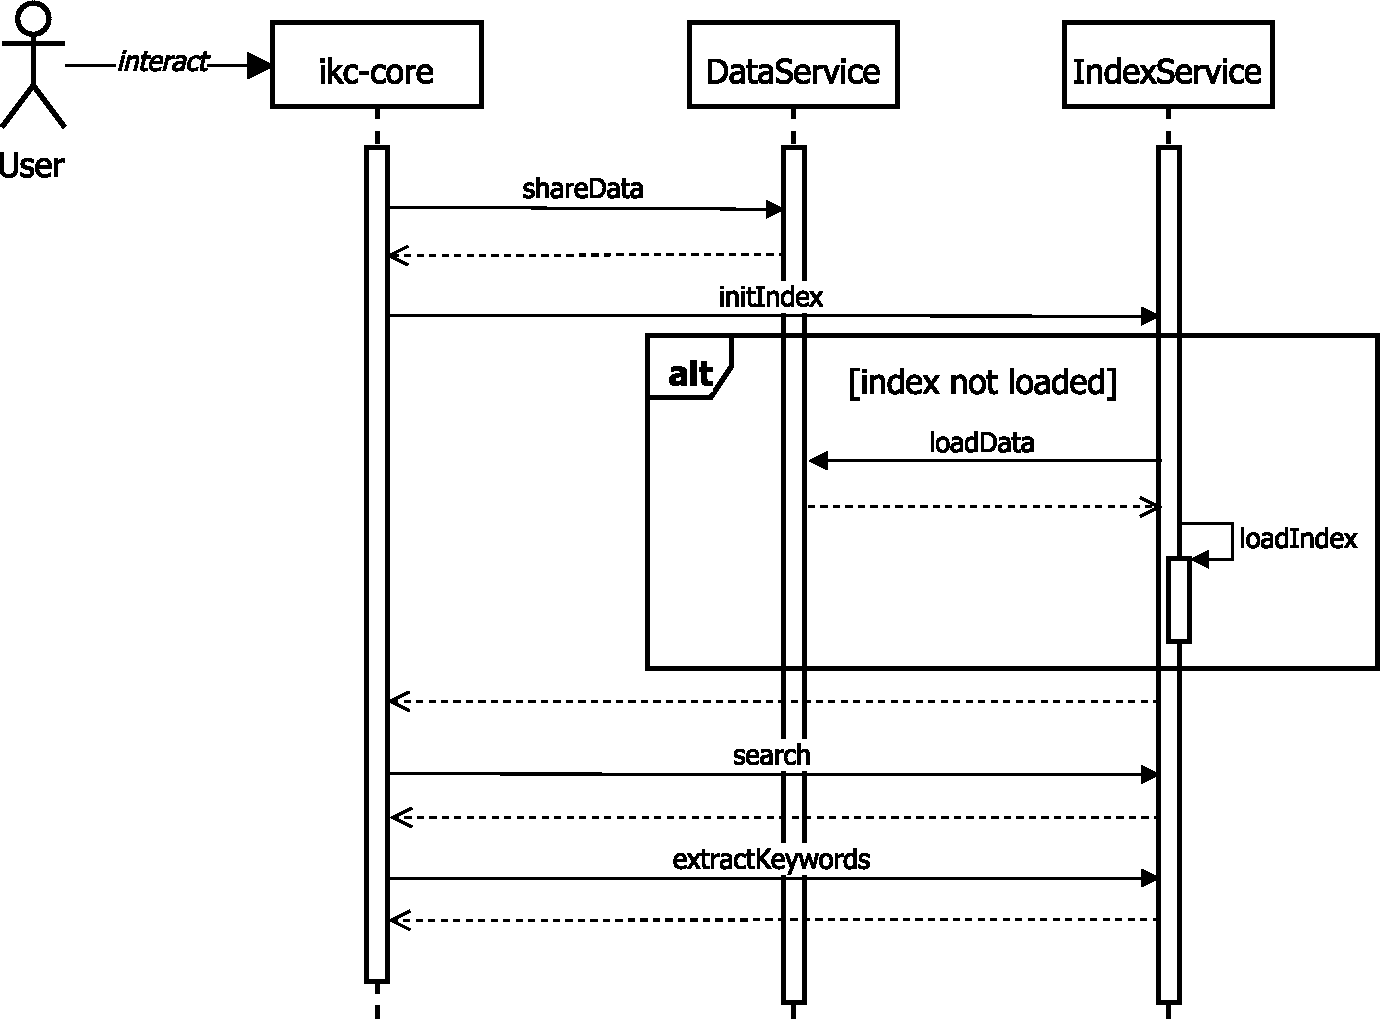
\includegraphics[width=1\textwidth]{BDA_Sequence}
\caption{Ablaufsicht}
\label{fig:ablaufsicht}
\end{figure}

Die erhaltene Freigabe gibt der \gls{ikc-core} im Prozess \texttt{initIndex} an den \texttt{IndexService} weiter. Hat dieser den angeforderten Index bereits geladen, gibt er diesen an den \gls{ikc-core} zurück. Ist dies nicht der Fall, holt er sich beim \texttt{Data\-Service} wiederum die benötigten Daten (\texttt{loadData}). Diese können denselben Inhalt wie oben haben. Das ist abhängig davon, ob der Index bereits erstellt wurde. Ist dies nicht der Fall, muss dieser auf Basis aller Dateien erstellt werden. Ist er bereits erstellt, oder spätestens nach dessen Erstellung, wird dies an den \gls{ikc-core} gemeldet.

Nun kann der \gls{ikc-core} die Funktionalität des \texttt{IndexService} nutzen: Er hat Zugriff auf die Volltextsuche (\texttt{search}) und die extrahierten Schlüsselwörter (\texttt{extractKeywords}). 


%---------------------------------------------------------------------

\subsection{Verteilung}

%---------------------------------------------------------------------

Wie oben schon angesprochen, findet die Entwicklung sowohl client- als auch serverseitig statt. \autoref{fig:verteilung} gibt einen detaillierten Üb\-er\-blick. Auf der Seite des Clients läuft der \gls{ikc-core} im Browser. Dieser verwendet für die Zwischenspeicherung von Daten eine \gls{in-browser Datenbank}.

    
        \begin{figure}[H]
    \centering
    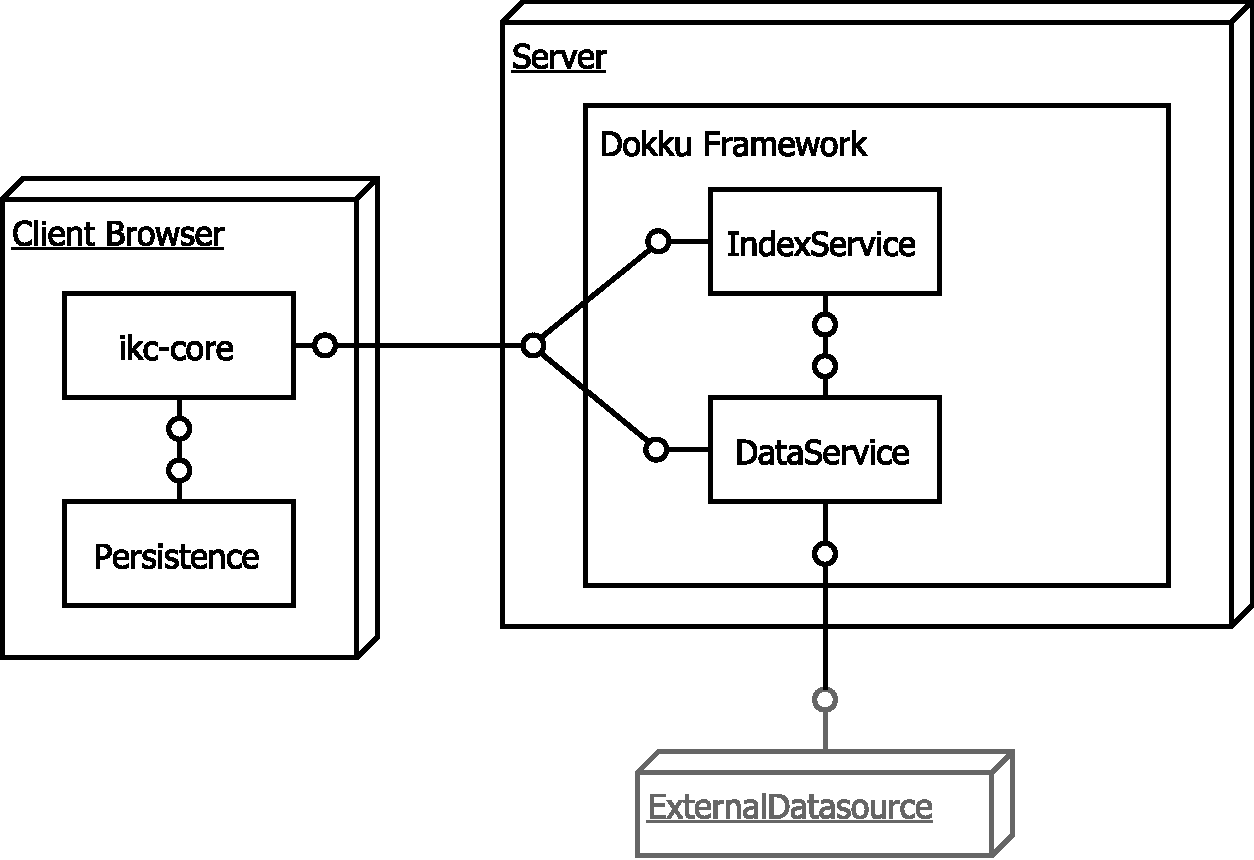
\includegraphics[width=0.7\textwidth]{DistributionView}
    \caption{Verteilung}
    \label{fig:verteilung}
    \end{figure}
